% ****************************************************************************************
% ************************      REPORTE DE BASE DE DATOS     *****************************
% ****************************************************************************************

%  =======================================================
% =======         HEADER FOR DOCUMENT        ============
% =======================================================
    % *********   DOCUMENT ITSELF   **************
    \documentclass[12pt, fleqn]{article}                             %Type of docuemtn and size of font and left eq
    \usepackage[margin=1.2in]{geometry}                             %Margins and Geometry pacakge
    \usepackage{ifthen}                                             %Allow simple programming
    \usepackage{hyperref}                                           %Create MetaData for a PDF and LINKS!
    \hypersetup{pageanchor=false}                                   %Solve 'double page 1' warnings in build
    \setlength{\parindent}{0pt}                                     %Eliminate ugly indentation
    \author{Oscar Andrés Rosas}                                     %Who I am

    % *********   LANGUAJE AND UFT-8   *********
    \usepackage[spanish]{babel}                                     %Please use spanish
    \usepackage[utf8]{inputenc}                                     %Please use spanish - UFT
    \usepackage[T1]{fontenc}                                        %Please use spanish
    \usepackage{textcmds}                                           %Allow us to use quoutes
    \usepackage{changepage}                                         %Allow us to use identate paragraphs
    \usepackage{lipsum}                                             %Allow to put dummy text

    % *********   MATH AND HIS STYLE  *********
    \usepackage{ntheorem, amsmath, amssymb, amsfonts}               %All fucking math, I want all!
    \usepackage{mathrsfs, mathtools, empheq}                        %All fucking math, I want all!
    \usepackage{centernot}                                          %Allow me to negate a symbol
    \decimalpoint                                                   %Use decimal point

    % *********   GRAPHICS AND IMAGES *********
    \usepackage{graphicx}                                           %Allow to create graphics
    \usepackage{wrapfig}                                            %Allow to create images
    \graphicspath{ {Graphics/} }                                    %Where are the images :D

    % *********   LISTS AND TABLES ***********
    \usepackage{listings}                                           %We will be using code here
    \usepackage[inline]{enumitem}                                   %We will need to enumarate
    \usepackage{tasks}                                              %Horizontal lists
    \usepackage{longtable}                                          %Lets make tables awesome
    \usepackage{booktabs}                                           %Lets make tables awesome
    \usepackage{tabularx}                                           %Lets make tables awesome
    \usepackage{multirow}                                           %Lets make tables awesome
    \usepackage{multicol}                                           %Create multicolumns

    % *********   HEADERS AND FOOTERS ********
    \usepackage{fancyhdr}                                           %Lets make awesome headers/footers
    \pagestyle{fancy}                                               %Lets make awesome headers/footers
    \setlength{\headheight}{16pt}                                   %Top line
    \setlength{\parskip}{0.5em}                                     %Top line
    \renewcommand{\footrulewidth}{0.5pt}                            %Bottom line

    \lhead{                                                         %Left Header
        \hyperlink{section.\arabic{section}}                        %Make a link to the current chapter
        {\normalsize{\textsc{\nouppercase{\leftmark}}}}             %And fot it put the name
    }

    \rhead{                                                         %Right Header
        \hyperlink{section.\arabic{section}.\arabic{subsection}}    %Make a link to the current chapter
            {\footnotesize{\textsc{\nouppercase{\rightmark}}}}      %And fot it put the name
    }

    \rfoot{\textsc{\small{Practica 1 y 2}}}                          %This will always be a footer  

    \fancyfoot[L]{                                                  %Algoritm for a changing footer
        \ifthenelse{\isodd{\value{page}}}                           %IF ODD PAGE:
            {\href{https://compilandoconocimiento.com/yo/}          %DO THIS:
                {\footnotesize                                      %Send the page
                    {\textsc{Oscar Andrés Rosas}}}}                 %Send the page
            {\href{https://compilandoconocimiento.com}              %ELSE DO THIS: 
                {\footnotesize                                      %Send the author
                    {\textsc{Compilando Conocimiento}}}}            %Send the author
    }
    
    
    
% ========================================
% ===========   COMMANDS    ==============
% ========================================

    % =====  GENERAL TEXT  ==========
    \newcommand \Quote {\qq}                                        %Use: \Quote to use quotes
    \newcommand \Over {\overline}                                   %Use: \Bar to use just for short
    \newcommand \ForceNewLine {$\Space$\\}                          %Use it in theorems for example
    
    \newenvironment{Indentation}[1][0.75em]                         %Use: \begin{Inde...}[Num]...\end{Inde...}
    {\begin{adjustwidth}{#1}{}}                                     %If you dont put nothing i will use 0.75 em
    {\end{adjustwidth}}                                             %This indentate a paragraph
    \newenvironment{SmallIndentation}[1][0.75em]                    %Use: The same that we upper one, just 
    {\begin{adjustwidth}{#1}{}\begin{footnotesize}}                 %footnotesize size of letter by default
    {\end{footnotesize}\end{adjustwidth}}                           %that's it
        
    % =====  GENERAL MATH  ==========
    \DeclareMathOperator \Space {\quad}                             %Use: \Space for a cool mega space
    \DeclareMathOperator \MiniSpace {\;}                            %Use: \Space for a cool mini space
    \newcommand \Such {\MiniSpace|\MiniSpace}                       %Use: \Such like in sets
    \newcommand \Also {\Space \text{y} \Space}                      %Use: \Also so it's look cool
    \newcommand \Remember[1]{\Space\text{\scriptsize{#1}}}          %Use: \Remember so it's look cool

    \newtheorem{Theorem}{Teorema}[section]                          %Use: \begin{Theorem}[Name]\label{Nombre}...
    \newtheorem{Corollary}{Colorario}[Theorem]                      %Use: \begin{Corollary}[Name]\label{Nombre}...
    \newtheorem{Lemma}[Theorem]{Lemma}                              %Use: \begin{Lemma}[Name]\label{Nombre}...
    \newtheorem{Definition}{Definición}[section]                    %Use: \begin{Definition}[Name]\label{Nombre}...

    \newcommand{\Set}[1]{\left\{ \MiniSpace #1 \MiniSpace \right\}} %Use: \Set {Info}
    \newcommand{\Brackets}[1]{\left[ #1 \right]}                    %Use: \Brackets {Info} 
    \newcommand{\Wrap}[1]{\left( #1 \right)}                        %Use: \Wrap {Info} 
    \newcommand{\pfrac}[2]{\Wrap{\dfrac{#1}{#2}}}                   %Use: Put fractions in parentesis

    \newenvironment{MultiLineEquation}[1]                           %Use: To create MultiLine equations
        {\begin{equation}\begin{alignedat}{#1}}                     %Use: \begin{Multi..}{Num. de Columnas}
        {\end{alignedat}\end{equation}}                             %And.. that's it!
    \newenvironment{MultiLineEquation*}[1]                          %Use: To create MultiLine equations
        {\begin{equation*}\begin{alignedat}{#1}}                    %Use: \begin{Multi..}{Num. de Columnas}
        {\end{alignedat}\end{equation*}}                            %And.. that's it!


    % =====  LOGIC  ==================
    \DeclareMathOperator \doublearrow {\leftrightarrow}             %Use: \doublearrow for a double arrow
    \newcommand \lequal {\MiniSpace \Leftrightarrow \MiniSpace}     %Use: \lequal for a double arrow
    \newcommand \linfire {\MiniSpace \Rightarrow \MiniSpace}        %Use: \lequal for a double arrow
    \newcommand \longto {\longrightarrow}                           %Use: \longto for a long arrow

    % =====  NUMBER THEORY  ==========
    \DeclareMathOperator \Naturals  {\mathbb{N}}                     %Use: \Naturals por Notation
    \DeclareMathOperator \Primes    {\mathbb{P}}                     %Use: \Naturals por Notation
    \DeclareMathOperator \Integers  {\mathbb{Z}}                     %Use: \Integers por Notation
    \DeclareMathOperator \Racionals {\mathbb{Q}}                     %Use: \Racionals por Notation
    \DeclareMathOperator \Reals     {\mathbb{R}}                     %Use: \Reals por Notation
    \DeclareMathOperator \Complexs  {\mathbb{C}}                     %Use: \Complex por Notation

    % === LINEAL ALGEBRA & VECTORS ===
    \DeclareMathOperator \LinealTransformation {\mathcal{T}}        %Use: \LinealTransformation for a cool T
    \newcommand{\Mag}[1]{\left| #1 \right|}                         %Use: \Mag {Info} 

    \newcommand{\pVector}[1]{                                       %Use: \pVector {Matrix Notation} use parentesis
        \ensuremath{\begin{pmatrix}#1\end{pmatrix}}                 %Example: \pVector{a\\b\\c} or \pVector{a&b&c} 
    }
    \newcommand{\lVector}[1]{                                       %Use: \lVector {Matrix Notation} use a abs 
        \ensuremath{\begin{vmatrix}#1\end{vmatrix}}                 %Example: \lVector{a\\b\\c} or \lVector{a&b&c} 
    }
    \newcommand{\bVector}[1]{                                       %Use: \bVector {Matrix Notation} use a brackets 
        \ensuremath{\begin{bmatrix}#1\end{bmatrix}}                 %Example: \bVector{a\\b\\c} or \bVector{a&b&c} 
    }
    \newcommand{\Vector}[1]{                                        %Use: \Vector {Matrix Notation} no parentesis
        \ensuremath{\begin{matrix}#1\end{matrix}}                   %Example: \Vector{a\\b\\c} or \Vector{a&b&c}
    }

    % MATRIX
    \makeatletter                                                   %Example: \begin{matrix}[cc|c]
    \renewcommand*\env@matrix[1][*\c@MaxMatrixCols c] {             %WTF! IS THIS
        \hskip -\arraycolsep                                        %WTF! IS THIS
        \let\@ifnextchar\new@ifnextchar                             %WTF! IS THIS
        \array{#1}                                                  %WTF! IS THIS
    }                                                               %WTF! IS THIS
    \makeatother                                                    %WTF! IS THIS

    % TRIGONOMETRIC FUNCTIONS
    \newcommand{\Cos}[1]{\cos\Wrap{#1}}                             %Simple wrappers
    \newcommand{\Sin}[1]{\sin\Wrap{#1}}                             %Simple wrappers

    % === COMPLEX ANALYSIS ===
    \newcommand \Cis[1]  {\Cos{#1} + i \Sin{#1}}                    %Use: \Cis for cos(x) + i sin(x)
    \newcommand \pCis[1] {\Wrap{\Cis{#1}}}                          %Use: \pCis for the same ut parantesis
    \newcommand \bCis[1] {\Brackets{\Cis{#1}}}                      %Use: \bCis for the same to Brackets




% =====================================================
% ============        COVER PAGE       ================
% =====================================================
\begin{document}
\begin{titlepage}

    \center
    % ============ UNIVERSITY NAME AND DATA =========
    \textsc{\Large ESCOM - IPN}\\[0.5cm] 
    \textsc{\large Bases de Datos 2CM12}\\[1.5cm]

    % ============ NAME OF THE DOCUMENT  ============
    \rule{\linewidth}{0.5mm} \\[1.0cm]
        { \huge \bfseries Introducción a las Bases de Datos}\\[1.0cm] 
    \rule{\linewidth}{0.5mm} \\[2.0cm]
     
    % ============  MY INFORMATION  =================
    \begin{minipage}{0.4\textwidth}
        \begin{flushleft} \large
            \textbf{\textsc{Alumno:}}\\
            Rosas Hernandez Oscar Andres
        \end{flushleft}
    \end{minipage}
    ~
    \begin{minipage}{0.4\textwidth}
        \begin{flushright} \large
            \textbf{\textsc{Profesor: }}\\
            Euler Hernandez Contreras
        \end{flushright}
    \end{minipage}\\[3,5cm]

    % ====== SEMI TITLE ==========
    {\LARGE Reporte 1 y Reporte 2}\\[4cm] 
    
    
    \vfill

\end{titlepage}









% ===============================================================================
% ===================           PARTE TEORICA              ======================
% ===============================================================================
\section{Parte Teórica}

    ¿Cómo se almacenan grandes colecciones de datos en constante cambio en disco?
    ¿Cómo podemos hacer que diferentes agentes recuperen, editen y agreguen datos al mismo tiempo?

    En lugar de implementar estas funcionalidades nosotros mismos, usaremos una
    DataBase Management System (DBMS).
    Una pieza especial de software para administrar bases de datos.
    El DBMS organiza y almacena los datos. Mediace los accesos y los cambios en la base de datos.



    \subsection{Introducción}

        Las bases de datos relacionales facilitan evitar la duplicidad de información
        e inconsistencias de datos.
        La mayoría de los sistemas de bases de datos utilizados hoy en día son relacionales.

        En el modelo relacional, los datos se dividen en diferentes \textbf{tables}.
        Una tabla funciona como una matriz o una hoja de cálculo.

        Normalmente, las columnas imponen un tipo de datos que pueden contener.
        Las columnas también pueden especificar otras restricciones: si es obligatorio que las
        filas tengan un valor en esa columna, si el valor de la columna debe ser único en todas
        las filas y cosas así.

        Las columnas se denominan más comúnmente atributos.
        Si una columna sólo permite números enteros, decimos que es un campo entero.
        Diferentes tablas utilizan diferentes tipos de campos.

        La organización de una tabla de base de datos viene dada por sus campos y las
        restricciones que imponen.

        Todas las entradas de datos son filas y el sistema de base de datos no aceptará
        una fila en una tabla si viola el esquema de la tabla. Esa es una gran limitación
        del modelo relacional.
        Cuando las características de los datos varían demasiado, la adaptación de los datos
        a un esquema fijo puede ser problemática. Pero si está trabajando con datos de
        estructura homogénea, un esquema fijo le ayudará a garantizar que los datos son válidos.

        \clearpage
        \subsubsection{Relaciones}

            Para evitar la redundancia de datos la clave esta en crear diversas tablas
            e ir relacionandolas.

            Para lograr esto tenemos que crear relaciones, y es imposible hablar de relaciones
            sin hablar de llaves:


            \begin{itemize}
                \item
                    \textbf{Primary Key:}
                    La idea de una llave primaria es crear un atributo que tiene, tiene pero
                    tiene que ser único y es recomendable que casi no cambie.


                \item
                    \textbf{Foreign Key:}
                    La idea de una llave secundaria es crear un atributo que tiene que alguna otra
                    tabla sea la llave primaria. Eso es todo.

            \end{itemize}


    \subsection{SQL como Lenguaje}
        
        SQL \textbf{no} es tan potente como una máquina universal de Turing.

        Es decir, hay algunos cálculos que son posibles utilizando un lenguaje de programación
        de propósito general, pero no son posibles con SQL.
        SQL también no admite acciones como la entrada de usuarios, la salida a las pantallas 
        ó la comunicación a través de la red.
        Dichas computaciones y acciones deben escribirse en un lenguaje principal (C, C++ ó Java)
        con consultas SQL incorporadas que acceden a los datos de la base de datos

        Los programas de aplicación son programas que se utilizan para interactuar con la base de
        datos de esta manera.



% ===============================================================================
% ===================           MARCO PRACTICO             ======================
% ===============================================================================
\clearpage
\section{Parte Practica: Practica 1}

    Veamor por pasos que es lo que hicimos:

    \begin{itemize}

        \item
            \textbf{Crear la Base de Datos:}
            \lstset{basicstyle=\tiny}
            \lstinputlisting[language=SQL]{Snippets/Snippet0.sql}

        \item
            \textbf{Construimos las Relaciones Propietarias:}
            \lstset{basicstyle=\tiny}
            \lstinputlisting[language=SQL]{Snippets/Snippet1.sql}
            
        \clearpage
        \item{Alteramos las Relaciones}
            Es decir, vamos a hacer lo siguiente:
            
            \begin{itemize}
                \item Renombrar las Relación Profesor a Catedratico
                \item Agregar un campo a la relación Presentacion
                \item Cambiar el Nombre de Departamento
                \item Agregar telefono del Catedratico
                \item Cambiar el tipo de dato del Tel. del Catedratico
            \end{itemize}
            
            \lstset{basicstyle=\tiny}
            \lstinputlisting[language=SQL]{Snippets/Snippet2.sql}


        \item
            \textbf{Agregar Foreign Key:}
            \lstset{basicstyle=\tiny}
            \lstinputlisting[language=SQL]{Snippets/Snippet3.sql}
            
        \item
            \textbf{Cambiar la definición de la PK en Presentación:}
            \lstset{basicstyle=\tiny}
            \lstinputlisting[language=SQL]{Snippets/Snippet4.sql}

    \end{itemize}


    % ================================================================
    % ===================       EVIDENCIAS           =================
    % ================================================================
    \clearpage
    \subsection{Evidencias}

        \begin{figure}[h]
            \centering
            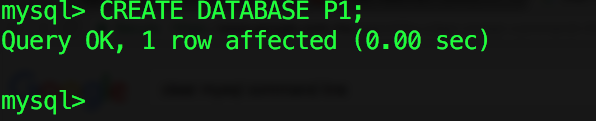
\includegraphics[width=0.45\textwidth]{BD1Reporte0}
            \caption{Empecemos por crear la BD}
        \end{figure}

        \begin{figure}[h]
            \centering
            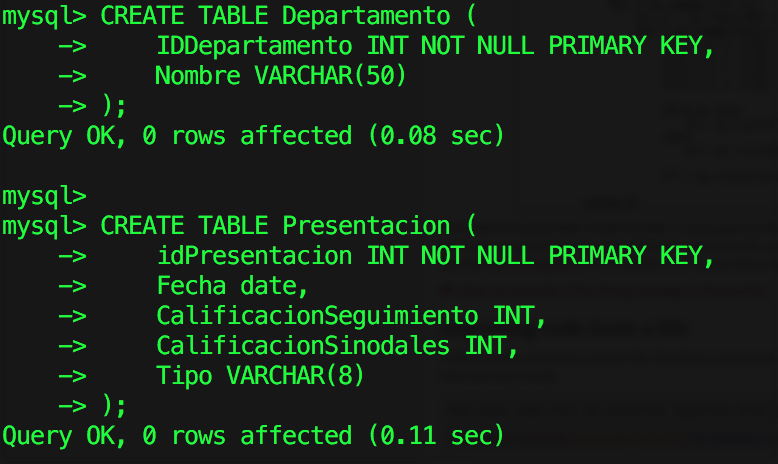
\includegraphics[width=0.85\textwidth]{BD1Reporte1}
            \caption{Creando tables}
        \end{figure}

        \begin{figure}[h]
            \centering
            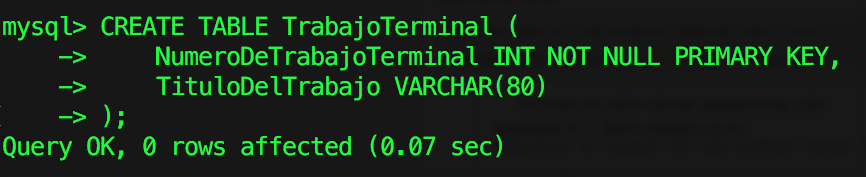
\includegraphics[width=0.85\textwidth]{BD1Reporte2}
            \caption{Creando tables}
        \end{figure}

        \begin{figure}[h]
            \centering
            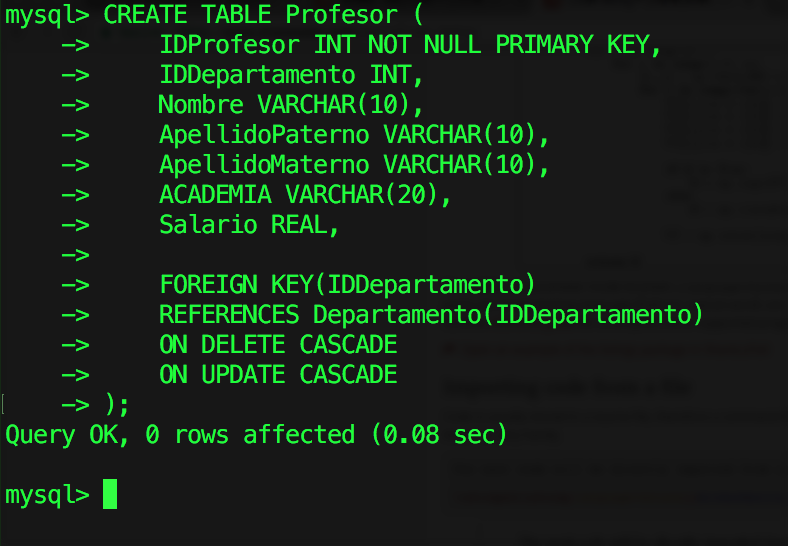
\includegraphics[width=0.85\textwidth]{BD1Reporte3}
            \caption{Creando tables}
        \end{figure}

        \begin{figure}[h]
            \centering
            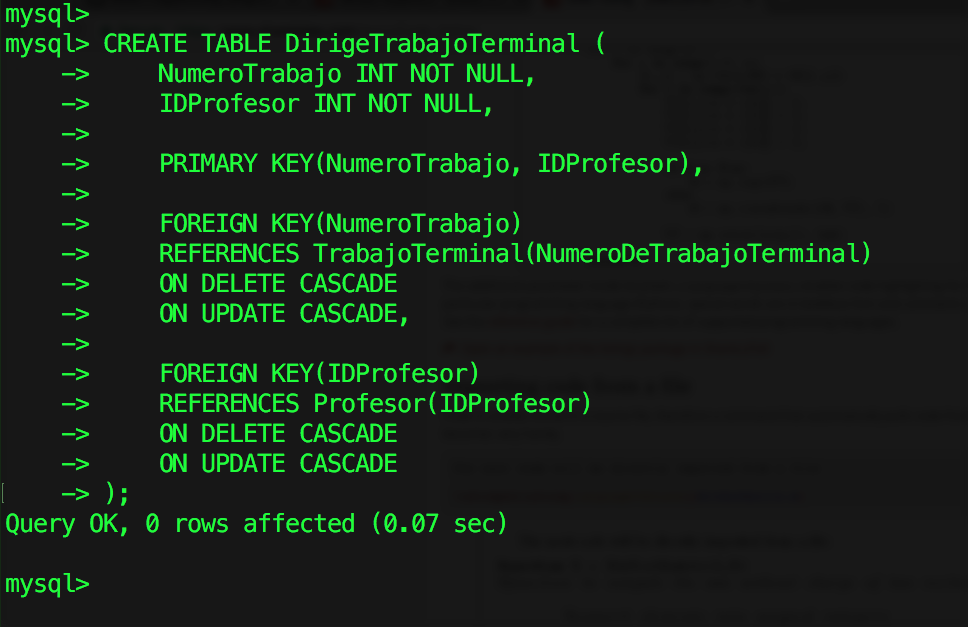
\includegraphics[width=0.85\textwidth]{BD1Reporte4}
            \caption{Creando tables}
        \end{figure}

        \begin{figure}[h]
            \centering
            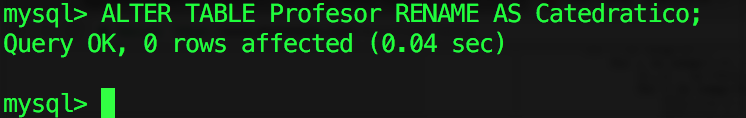
\includegraphics[width=0.85\textwidth]{BD1Reporte5}
            \caption{Modificandolas}
        \end{figure}

        \begin{figure}[h]
            \centering
            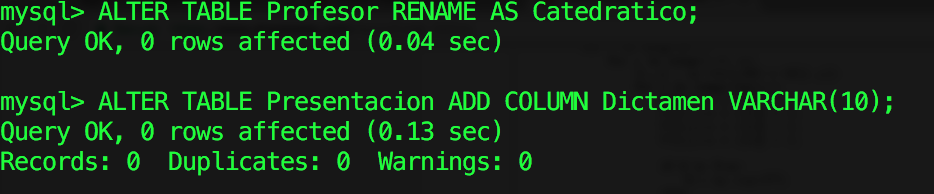
\includegraphics[width=0.85\textwidth]{BD1Reporte6}
            \caption{Modificandolas}
        \end{figure}

        \begin{figure}[h]
            \centering
            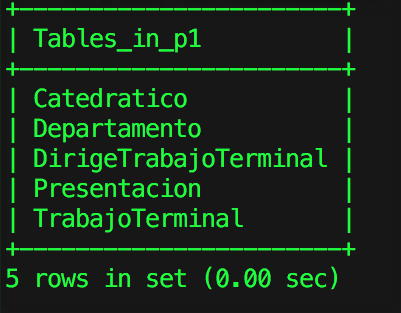
\includegraphics[width=0.45\textwidth]{BD1Reporte7}
            \caption{Veamos las tablas que tenemos}
        \end{figure}


        \begin{figure}[h]
            \centering
            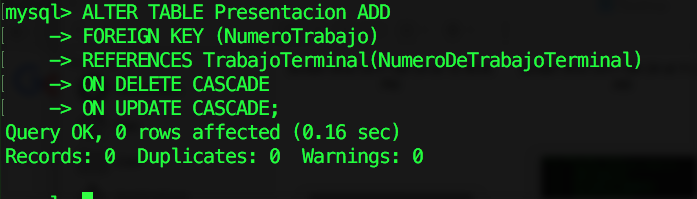
\includegraphics[width=0.85\textwidth]{BD1Reporte8}
            \caption{Modificandolas}
        \end{figure}

        \clearpage

        \begin{figure}[h!]
            \centering
            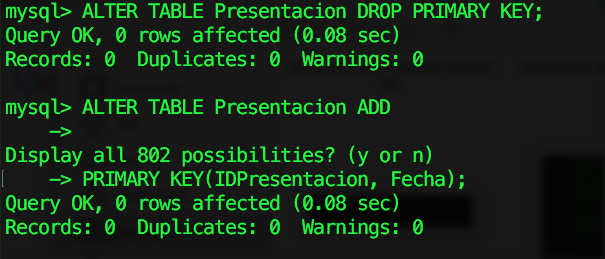
\includegraphics[width=0.85\textwidth]{BD1Reporte9}
            \caption{Modificamos las Key}
        \end{figure}







% ===============================================================================
% ===================           MARCO PRACTICO             ======================
% ===============================================================================
\clearpage
\section{Parte Practica: Practica 2}

    Veamor por pasos que es lo que hicimos:

    \begin{itemize}

        \item
            \textbf{Crear las relaciones del nuevo ejercicio:}
            \lstset{basicstyle=\tiny}
            \lstinputlisting[language=SQL]{Snippets/Snippet5.sql}

        \item
            \textbf{Modificamos un poco las relaciones:}
            \lstset{basicstyle=\tiny}
            \lstinputlisting[language=SQL]{Snippets/Snippet6.sql}

        \item
            \textbf{Añadamos la relación gerente:}
            \lstset{basicstyle=\tiny}
            \lstinputlisting[language=SQL]{Snippets/Snippet7.sql}

        \item
            \textbf{Modifiquemos un poco las relaciones:}
            \lstset{basicstyle=\tiny}
            \lstinputlisting[language=SQL]{Snippets/Snippet8.sql}
            
        \clearpage
        \item{Vamos a Cambiar una Llave Primaria}
            Es decir, vamos a hacer lo siguiente:
            
            \begin{itemize}
                \item
                    Eliminar las LLaves Foraneas de EmpleadoCinemex y Gerente

                    \lstset{basicstyle=\tiny}
                    \lstinputlisting[language=SQL]{Snippets/Snippet90.sql}

                \item
                    Buscamos el Contraint

                    \lstset{basicstyle=\tiny}
                    \lstinputlisting[language=SQL]{Snippets/Snippet91.sql}

                    \lstset{basicstyle=\tiny}
                    \lstinputlisting[language=SQL]{Snippets/Snippet92.sql}


                \item
                    Eliminar la llave primaria y Coloca una nueva llave primaria

                    \lstset{basicstyle=\tiny}
                    \lstinputlisting[language=SQL]{Snippets/Snippet93.sql}

                \item
                    Añadir campos necesarios y unirlos

                    \lstset{basicstyle=\tiny}
                    \lstinputlisting[language=SQL]{Snippets/Snippet94.sql}

            \end{itemize}


        \item
            \textbf{Añadamos otra relación:}
            \lstset{basicstyle=\tiny}
            \lstinputlisting[language=SQL]{Snippets/Snippet10.sql}

        \clearpage

        \item
            \textbf{Añadamos una Base externa:}
            \lstset{basicstyle=\tiny}
            \lstinputlisting[language=SQL]{Snippets/Snippet100.sql}
            
        \item
            \textbf{Veamos la información de dicha base:}
            \lstset{basicstyle=\tiny}
            \lstinputlisting[language=SQL]{Snippets/Snippet101.sql}


    \end{itemize}



    % ================================================================
    % ===================       EVIDENCIAS           =================
    % ================================================================
    \clearpage
    \subsection{Evidencias}

        \begin{figure}[h]
            \centering
            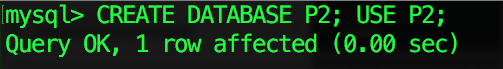
\includegraphics[width=0.45\textwidth]{BD2Reporte0}
            \caption{Creamos la base de datos}
        \end{figure}

        \begin{figure}[h]
            \centering
            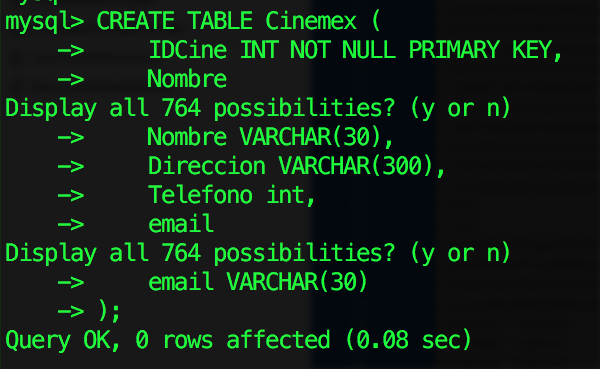
\includegraphics[width=0.45\textwidth]{BD2Reporte1}
            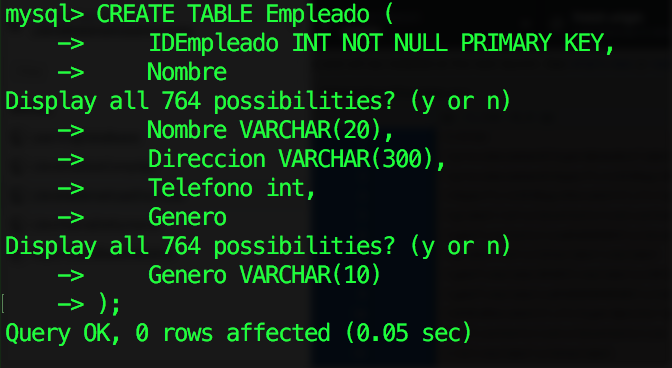
\includegraphics[width=0.45\textwidth]{BD2Reporte2}
            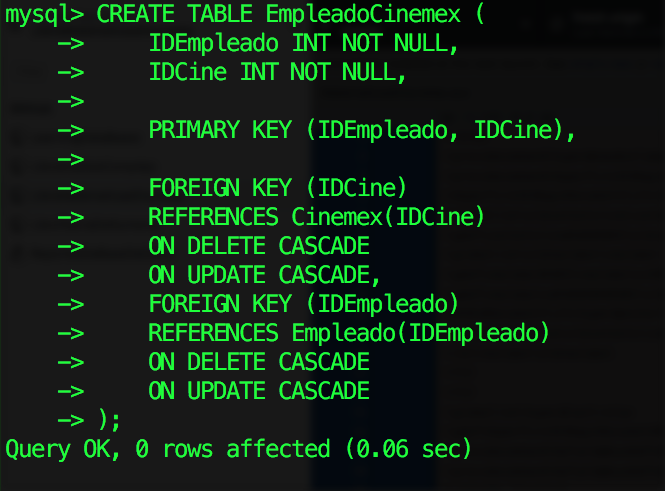
\includegraphics[width=0.45\textwidth]{BD2Reporte3}
            \caption{Creando tables}
        \end{figure}

        \begin{figure}[h]
            \centering
            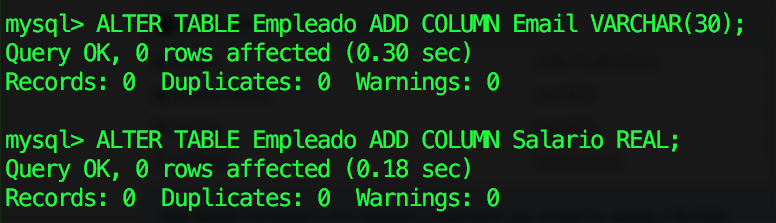
\includegraphics[width=0.85\textwidth]{BD2Reporte4}
            \caption{Modifiquemos un poco las tablas}
        \end{figure}

        \begin{figure}[h]
            \centering
            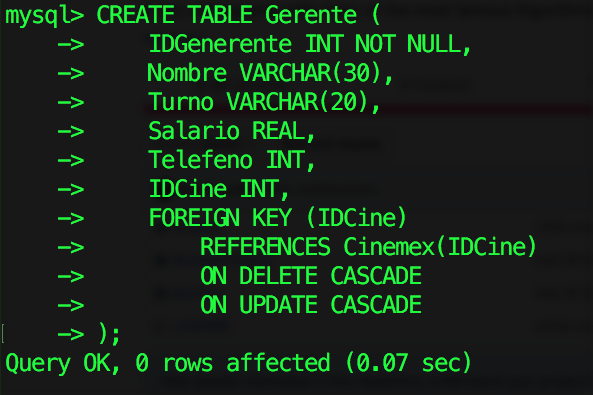
\includegraphics[width=0.85\textwidth]{BD2Reporte5}
            \caption{Creando tables}
        \end{figure}


        \begin{figure}[h]
            \centering
            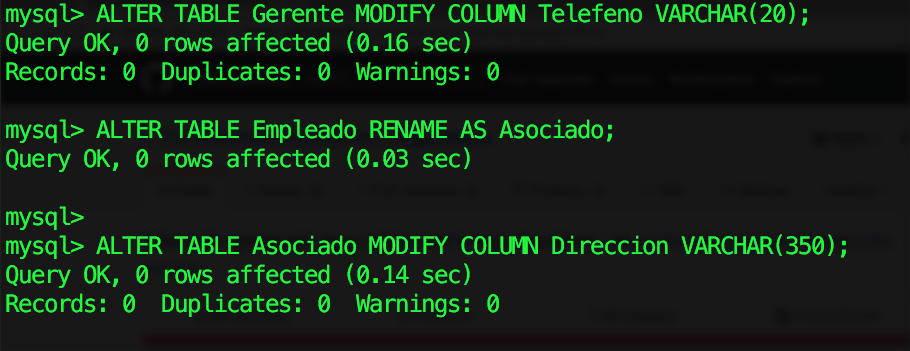
\includegraphics[width=0.85\textwidth]{BD2Reporte6}
            \caption{Creando tables}
        \end{figure}


        \begin{figure}[h]
            \centering
            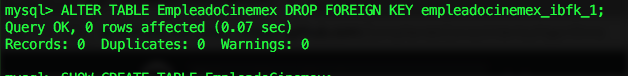
\includegraphics[width=0.85\textwidth]{BD2Reporte9}
            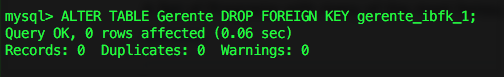
\includegraphics[width=0.85\textwidth]{BD2Reporte10}
            \caption{Eliminar keys}
        \end{figure}



        \begin{figure}[h]
            \centering
            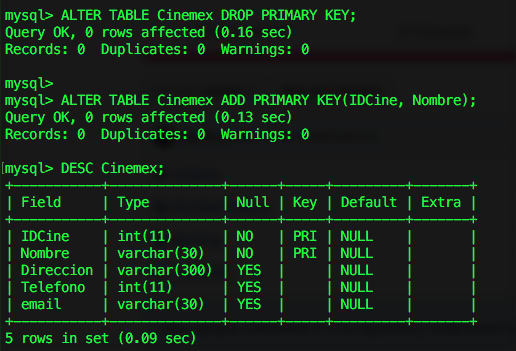
\includegraphics[width=0.85\textwidth]{BD2Reporte11}
            \caption{Añadimos una nueva llave primaria}
        \end{figure}


        \begin{figure}[h]
            \centering
            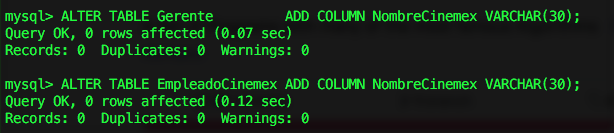
\includegraphics[width=0.85\textwidth]{BD2Reporte12}
            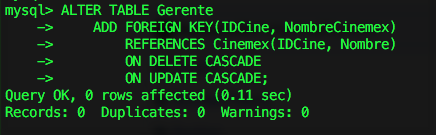
\includegraphics[width=0.65\textwidth]{BD2Reporte13}
            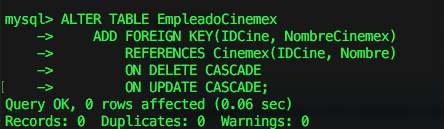
\includegraphics[width=0.65\textwidth]{BD2Reporte14}
            \caption{Las volvemos a unir}
        \end{figure}



        \begin{figure}[h]
            \centering
            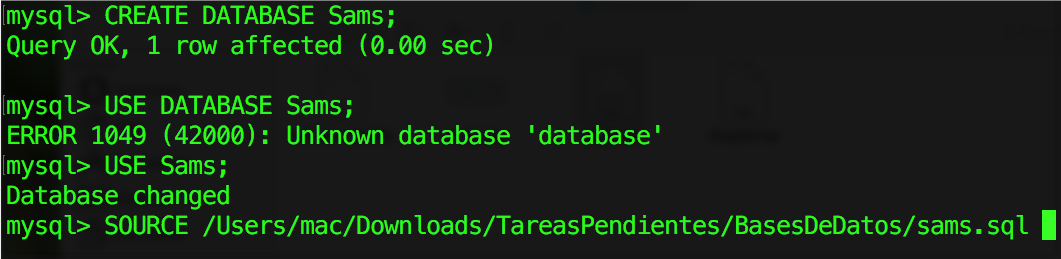
\includegraphics[width=0.65\textwidth]{DBExterna0}
            \caption{Creamos la nueva base y llenamos datos}
        \end{figure}

        \begin{figure}[h]
            \centering
            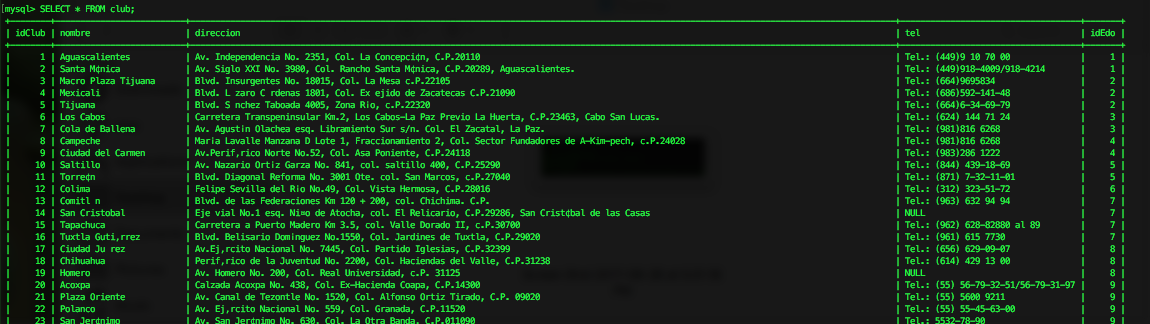
\includegraphics[width=0.85\textwidth]{DBExterna1}
            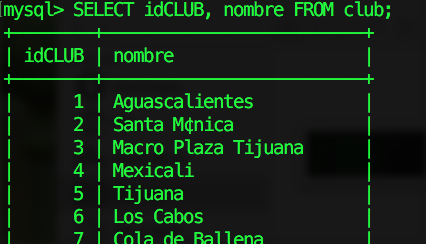
\includegraphics[width=0.55\textwidth]{DBExterna2}
            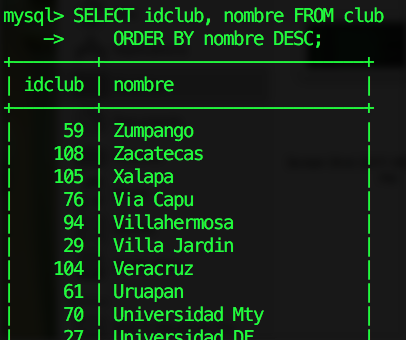
\includegraphics[width=0.45\textwidth]{DBExterna3}
            \caption{Veamos los datos}
        \end{figure}

        \clearpage


        \begin{figure}[h]
            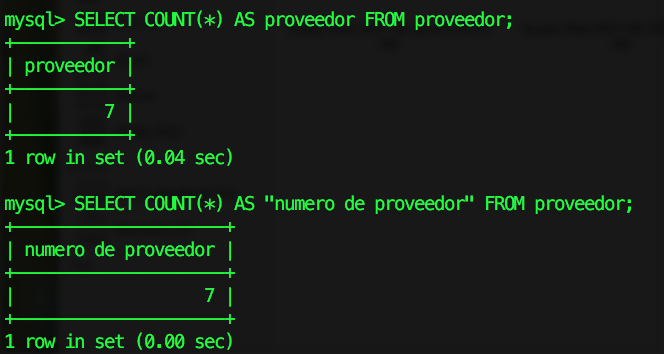
\includegraphics[width=0.45\textwidth]{DBExterna4}
            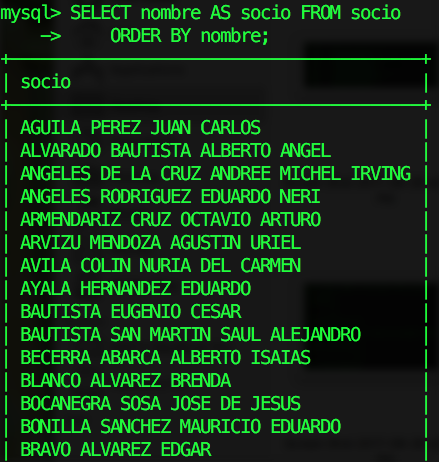
\includegraphics[width=0.45\textwidth]{DBExterna5}
            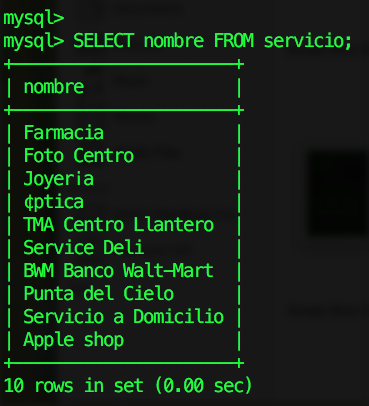
\includegraphics[width=0.45\textwidth]{DBExterna6}
            \caption{Veamos los datos}
        \end{figure}

        \begin{figure}[h]
            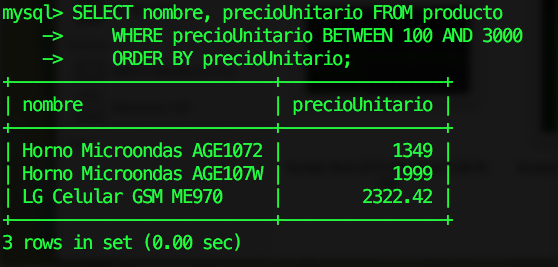
\includegraphics[width=0.45\textwidth]{DBExterna7}
            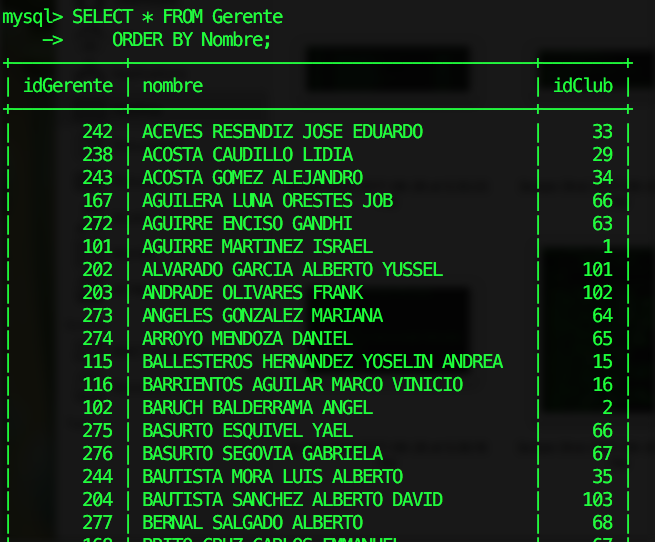
\includegraphics[width=0.45\textwidth]{DBExterna8}
            \caption{Veamos los datos}
        \end{figure}
        \clearpage
        




% ===============================================================================
% ===================           CONCLUSIONES               ======================
% ===============================================================================
\section{Conclusiones}

    Gracias a esta practica pudimos comprender mucho mejor como es que funcionan las bases de datos
    y lo facil que puede llegar a ser manipularlas para usarlas en sistemas computacionales.

    Aprendimos sobre el modelo relacional y como podemos separar nuestra informacion gracias a las tablas.
    Vimos como es que podemos volvera a unir gracias a las relaciones, el uso de llaves primarias y secundarias.





% =====================================================
% ============        BIBLIOGRAPHY   ==================
% =====================================================
\bibliographystyle{plain}
    \begin{thebibliography}{9}

    % ============ REFERENCE #1 ========
    \bibitem{Libro} 
        \texttt{Databases, Liberty Hall Chichester 1999}
        Bob Hudson

        \bibitem{Libro} 
        \texttt{Computer Science Distilled,}


     

\end{thebibliography}



\end{document}